%----------------------------------------------------------------------------------------
%	PACKAGES AND OTHER DOCUMENT CONFIGURATIONS
%----------------------------------------------------------------------------------------

% !TEX TS-program = pdflatex
% !TEX encoding = UTF-8 Unicode

% This is a simple template for a LaTeX document using the "article" class.
% See "book", "report", "letter" for other types of document.

\documentclass[11pt]{article} % use larger type; default would be 10pt
\usepackage[utf8]{inputenc}  % set input encoding (not needed with XeLaTeX)

%%% Examples of Article customizations
% These packages are optional, depending whether you want the features they provide.
% See the LaTeX Companion or other references for full information.

%%% PAGE DIMENSIONS
\usepackage{geometry}     % to change the page dimensions
\geometry{a4paper}          % or letterpaper (US) or a5paper or....
% \geometry{margin=2in} % for example, change the margins to 2 inches all round
% \geometry{landscape}   % set up the page for landscape
%  read geometry.pdf for detailed page layout information

%%% PACKAGES
\usepackage{booktabs}      % for much better looking tables
\usepackage{array}           % for better arrays (eg matrices) in maths
\usepackage{paralist}        % very flexible & customisable lists (eg. enumerate/itemize, etc.)
\usepackage{verbatim}      % adds environment for commenting out blocks of text & for better verbatim
\usepackage{subfig}          % make it possible to include more than one captioned figure/table in a single float
\usepackage{graphicx}       % support the \includegraphics command and options
\usepackage{siunitx}          % typesets SI units nicely
\usepackage{booktabs}      % allows for booktab tables
\graphicspath{ {images/} } % image file path
% \usepackage[parfill]{parskip} % Activate to begin paragraphs with an empty line rather than an indent
% These packages are all incorporated in the memoir class to one degree or another...
\usepackage{amsmath}  % for align environments

%%% HEADERS & FOOTERS
\usepackage{fancyhdr}                      % This should be set AFTER setting up the page geometry
\pagestyle{fancy}                              % options: empty , plain , fancy
\renewcommand{\headrulewidth}{0pt} % customise the layout...
\lhead{}\chead{}\rhead{}
\lfoot{}\cfoot{\thepage}\rfoot{}

%%% SECTION TITLE APPEARANCE
\usepackage{sectsty}
\allsectionsfont{\sffamily\mdseries\upshape} % (See the fntguide.pdf for font help)
% (This matches ConTeXt defaults)

%%% ToC (table of contents) APPEARANCE
\usepackage[nottoc,notlof,notlot]{tocbibind}                              % Put the bibliography in the ToC
\usepackage[titles,subfigure]{tocloft}                                       % Alter the style of the Table of Contents
\renewcommand{\cftsecfont}{\rmfamily\mdseries\upshape}
\renewcommand{\cftsecpagefont}{\rmfamily\mdseries\upshape} % No bold!

%%% END Article customizations

%%% The "real" document content comes below...

%----------------------------------------------------------------------------------------
%	TITLE SECTION 
%----------------------------------------------------------------------------------------

\title{The Thermodynamic Analysis of a Pratt \& Whitney F-100 Jet Engine}
\author{Team 11: Tanner Cooper, Hunter Ducharme, Melodi Felchak, Andrew Jurek}
\date{} % Activate to display a given date or no date (if empty),
              % otherwise the current date is printed 

\begin{document}
\maketitle

%----------------------------------------------------------------------------------------
%	INTRODUCTION
%----------------------------------------------------------------------------------------
\section{Introduction}

The purpose of this project is to analyze and better understand how a brayton cycle and jet engine work. Given information on the Pratt \& Whitney F-100 core and neglecting the turbofan, we defined two thermodynamic cycles for the engine: (1) the engine running at full throttle with no afterburner, and (2) the engine running on full throttle and full afterburner. We defined twenty-one stages in the first cycle and twenty-two in the second. The thrust produced by each cycle was also calculated. We evaluated the engine at an altitude of 6500 meters, under the cold air-standard and air-standard.

%----------------------------------------------------------------------------------------
%	GIVEN INFORMATION
%----------------------------------------------------------------------------------------
\section{Cycle Diagram and Given Information}
The following properties were known about the F-100 core before the analysis process.

\subsection{Compressor}
\begin{itemize}
\item Inlet area: $A_{\text{C}} = 0.5\ \si{m^{2}}$
\item Number of stages: $N_{\text{C}} = 0.5$
\item Interstage efficiency: $\eta_{\text{C}} = 0.97$
\item Overall pressure ratio: $P_{\text{C}} = 40$
\end{itemize}

\subsection{Combustor}
\begin{itemize}
\item Fuel type: JP-8
\item JP-8 calorific value: $Q_{\text{in}} = 43360\ \si{kJ/kg}$
\item Fuel mass flow rate: $\dot m_{\text{fuel 1}}\ (\si{kg/hr}) = 500 + 55 \dot m_{\text{inlet}}\ (\si{kg/s})$
\end{itemize}

\subsection{Turbine}
\begin{itemize}
\item Number of stages: $N_{\text{T}} = 4$
\item Interstage efficiency: $\eta_{\text{T}} = 0.92$
\end{itemize}

\subsection{Afterburner}
\begin{itemize}
\item Fuel mass flow rate: $\dot m_{\text{fuel 2}}\ (\si{kg/hr}) = -400 + 110 \dot m_{\text{inlet}}\ (\si{kg/s})$
\end{itemize}

\subsection{Nozzle}
\begin{itemize}
\item Exit area: $A_{\text{N}} = 0.3A_{\text{C}} = 0.150\ \si{m^2}$
\item Efficiency: $\eta_{\text{N}} = 0.92$
\end{itemize}


\subsection{Cycle Diagram}
\noindent Figure~\ref{fig:cycle_diagram} shows the cycle diagram of the F-100 core.

\begin{figure}[h!]
\centering
  \textbf{Figure 1} The Cyle Diagram\par\medskip
  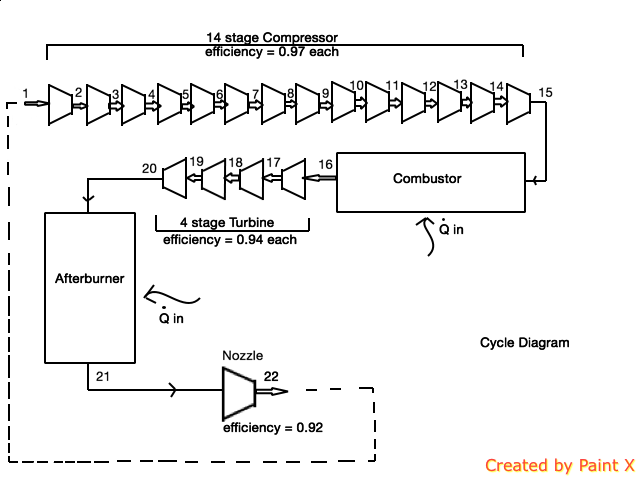
\includegraphics[scale=0.4]{cycle_diagram.png}
  \caption{This figure shows the locations of defined stages on a simplified model of the jet engine being analyzed. The dashed line represents the end of the cycle where the atmosphere would act as a heat exchanger to bring the temperature at stage 22 back down to the starting temperature, representing a true cycle.}
  \label{fig:cycle_diagram}
\end{figure}

%----------------------------------------------------------------------------------------
% ASSUMPTIONS
%----------------------------------------------------------------------------------------

\pagebreak
\section{Assumptions}

The assumptions that were made prior to analysis are listed below. The derivations of assumptions 2 and 6 can be found in the 'Derivations and Rationale' subsection.

\begin{enumerate}
\item Air is the working fluid and acts as an ideal gas.
\item There is no turbofan and and all ambient air goes straight to the compressor inlet.
\item The interstage pressure ratio across each stage of the compressor is constant.
\item The combustor and afterburner act as heat exchangers.
\item The combustor and afterburner work ideally (i.e. no pressure loss).
\item The backwork ratio of the cycle is one.
\item Each stage of the turbine produces the same amount of work.
\item Pressure at the inlet of the compressor is equal to the pressure at the exit of the nozzle.
\item All processes are internally reversible.
\end{enumerate}

\subsection*{Assumptions Specific to Air-standard}
None.

\subsection*{Assumptions Specific to Cold Air-standard}
\begin{enumerate}
\item $c_p = 1.005$, $c_{\upsilon} = 0.718$, and $k = 1.400$ are all constant throughout the cycle.
\item $h = c_pT$
\end{enumerate}

\subsection*{Derviations and Rationale}
For assumption 2, we assumed that each stage of the compressor will increase the pressure by the same multiple each time. To quantify this mathematically, suppose there exists a $\Delta P_i$ such that
\begin{align*}
P_n &= \Delta P_i P_{n-1} \\ \intertext{Therefore,}
P_{2} &= \Delta P_i P_{1} \\
P_{3} &= \Delta P_i P_{2} = (\Delta P_i)^2 P_{1} \\
\vdots \\
P_{n} &= (\Delta P_i)^{n-1} P_{1}. \\ \intertext{We can divide the pressure at state 15 by the pressure at state 1 to find $\Delta P_i$,}
\frac{P_{15}}{P_{1}} &= \frac{(\Delta P_i)^{14}P_{1}}{P_{1}} = (\Delta P_i)^{14}\\ \intertext{Therefore the interstage pressure ratio for the compressor is}
\Delta P_i &= \left(\frac{P_{15}}{P_{1}} \right)^{\frac{1}{14}} = (40)^{\frac{1}{14}} \approx 1.3015.
\end{align*}

For assumption 7, we assumed that each stage of the turbine produces the same amount of work. This means that 
\begin{align*}
W_n &= (h_{n-1} - h_n) = \text{constant}. \\ \intertext{So the enthalpies at each stage in the compressor are}
h_{17} &= h_{16} + \Delta h_i \\
h_{18} &= h_{17} + \Delta h_i = h_{16} + 2\Delta h_i \\
\vdots \\
h_{n} &= h_{n-1} + (\text{current turbine stage number})\Delta h_i. \\ \intertext{We can find $\Delta h_i$ by dividing the $h_{20}$ and $h_{16}$, where $h_{20}$ is found from using the backwork ratio of one (located in the analysis section)}
\frac{h_{20}}{h_{16}} &= \frac{h_{16} + 4\Delta h_i}{h_{16}} = 1 + \frac{4\Delta h_i}{h_{16}}. \\ \intertext{Therefore the enthalpy change across each stage of the turbine is}
\Delta h_i &= \frac{1}{4}h_{16}\left(\frac{h_{20}}{h_{16}} \right) -1) \approx -118.68 \si{kJ/kg}.
\end{align*}

%----------------------------------------------------------------------------------------
% ANALYSIS PROCEDURE
%----------------------------------------------------------------------------------------

\pagebreak
\section{Analysis Procedure}

In order to better understand thermodynamics and the calculation procedure itself, our team completed this project with both the cold air-standard procedure and the air-standard procedure. The steps taken for each procedure are shown below.

\subsection*{Cold Air-standard}
\subsubsection*{Compressor}
From assumption 2, the pressure ratio between stages of the compressor is constant, and the value (as shown above) is $\Delta P_i \approx 1.3015$. The temperatures could then be calculated using the isentropic relation

\begin{equation*}
T_{n} = T_{n-1}\left( \frac{P_n}{P_{n-1}} \right)^{ \frac{k-1}{k}},
\end{equation*}

\noindent where $n$ represents the stage number. Then, the ideal enthalpy from that with the enthalpy and temperature relation can be calculated using the ideal gas assumption that $\Delta h = c_p \Delta T$:

\begin{equation*}
h_{n} = c_pT_n.
\end{equation*}

\noindent Finally, the real enthalpy can be calculated from the compressor efficiency equation:

\begin{equation*}
\eta_{\text{C}} = \frac{ h_{ns} - h_{n-1} }{h_{n} - h_{n-1}}
\end{equation*}

\subsubsection*{Combustor}
Without a given efficiency value for the combustor, it is assumed to be acting ideally, resulting in no pressure change between stages 15 and 16 of the engine. The mass flow rates, and rate of heat addition in the combustor is the same in both the cold air-standard and the air-standard, and were calculated in the appendicies. \\

\noindent The equation 

\begin{equation*}
\frac{\dot{Q}_{\text{in combustor}}}{\dot{m}_{\text{out combustor}}} = h_{16} - h_{15}
\end{equation*}

\noindent was used to find the enthalpy at stage 16.

\subsubsection*{Turbine}
Assuming that the turbine produces the same amount of power that the compressor consumes, we know:

\begin{equation*}
\frac{\dot{W}_{\text{compressor}}}{\dot{m}_{\text{air}}} = h_{16} - h_{20} = \frac{\dot{W}_{\text{turbine}}}{\dot{m}_{\text{out combustor}}}
\end{equation*}

\noindent If we also assume that each stage of the turbine produces the same amount of work then the equation

\begin{equation*}
\Delta h = \frac{1}{4}(h_{16} - h_{20})
\end{equation*}

\noindent gives the change in enthalpy over each stage of the turbine. The isentropic enthalpies were found by

\begin{equation*}
\Delta h_{n+1} = \Delta h + h_n.
\end{equation*}

\noindent Then, the real enthalpies can be found from the turbine efficiency equation

\begin{equation*}
\eta_{\text{T}} = \frac{ h_{n} - h_{n-1} }{h_{ns} - h_{n-1}}
\end{equation*}

\subsubsection*{Afterburner}
Without a given efficiency value for the afterburner, it is assumed to be acting ideally. The mass flow rates, and rate of heat addition values are calculated in the appendicies. \\

\noindent The equation 

\begin{equation*}
\frac{\dot{Q}_{\text{in afterburner}}}{\dot{m}_{\text{out afterburner}}} = h_{21} - h_{20}
\end{equation*}

\noindent was used to find the enthalpy at stage 21.

\subsubsection*{Nozzle}
To find the exit velocity, the isentropic relation 

\begin{equation*}
T_{22} = T_{21}\left( \frac{P_{22}}{P_{21}} \right)^{ \frac{k-1}{k}},
\end{equation*}

\noindent was used to find the temperature at the exit of the nozzle. Then the enthalpy at stage 22 is found by the equation

\begin{equation*}
h_{22} = c_pT_{22}.
\end{equation*}

\noindent From there, the ideal exit velocity is calculated by

\begin{equation*}
V_{\text{es}} = \sqrt{2(h_{21} - h_{22})}.
\end{equation*}

\noindent The real velocity is then calculated using the nozzle efficiency equation:

\begin{equation*}
\eta_{\text{N}} = \frac{V_{\text{e}}^2}{V_{\text{es}}^2}
\end{equation*}

\noindent Note: In the first cycle, stage 21 is the same as stage 20, because the afterburner is not in use, so the values for stage 20 can be used in place of stage 21

\subsubsection*{Thrust}
The thrust for cyles 1 and 2 (with and without afterburner, respectively) is then calculated using the equations

\begin{align*}
T_{1} = \dot{m}_{\text{out combustor}}V_{e1}\\
T_{2} = \dot{m}_{\text{out afterburner}}V_{e2}\\.
\end{align*}

\subsection*{Air-standard}
\subsubsection*{Compressor}
From assumption 2, the pressure ratio between stages of the compressor is constant, and the value (as shown in the Assumptions section) is $\Delta P_i \approx 1.3015$. From this knowledge, the pressure at every state in the compressor is known, and thus the relative pressure at isentropic states can be found.

\noindent The alogrithim for solving the compressor is as follows: 
\begin{itemize}
\item Did we reach this state isentropically?
\begin{enumerate}
\item If yes, then calculate the relative pressure at this state using $P_{r_n} = P_{r_{n-1}} \Delta P_i$. Then every other property value can be interpolated, and most importantly the enthalpy can be found.
\item If no, then calculate the enthalpy using the interstage efficiency $\eta_{\text{C}} = \frac{ h_{ns} - h_{n-1} }{h_{n} - h_{n-1}}$. Then all other values at this state can be interpolated.
\end{enumerate}
\end{itemize}

\subsubsection*{Combustor}
The mass flow rates, and rate of heat addition in the combustor is the same in both the cold air-standard and the air-standard, and were calculated in the appendicies. \\

\noindent The enthalpy after the combustor (state 16) can be found using the 1st law of thermodynamics,

\begin{align*}
\frac{\dot{Q}_{\text{in combustor}}}{\dot{m}_{\text{out combustor}}} = h_{16} - h_{15} \\ \intertext{where}
\dot{Q}_{\text{in combustor}} = Q_{in}\dot{m}_{\text{fuel1}}
\end{align*}

\subsubsection*{Turbine}
From assumption 6, the enthalpy change across each stage of the turbine is constant, and the value (as shown in the Assumptions section) is $\Delta h \approx -118.68 \si{kJ/kg}.$ Since we know the enthalpy at state 16, we now know each enthalpy value at every real state in the turbine. 

\noindent The alogrithim for solving the turbine is as follows: 
\begin{enumerate}
\item Go to every real state in the turbine (i.e. 17, 18, 19, and 20)
\item Find the enthalpy at its resepective isentropic state (i.e. 17s, 18s, 19s, and 20s) using the interstage turbine efficiency $\eta_{\text{T}} = \frac{ h_{n} - h_{n-1} }{h_{ns} - h_{n-1}}$.
\item At the isentropic state, use the relative pressure equation $P_{r_n} = P_{r_{n-1}} \left( \frac{P_{n}}{P_{n-1}} \right)$ to find the pressure for both the isentropic state and the real state.
\item Once enthalpy at the real states, the enthalpy at the isentropic states, and the pressure at all states are known, every other property value can be found through interpolation.
\end{enumerate}


\subsubsection*{Afterburner}
The mass flow rates, and rate of heat addition in the combustor is the same in both the cold air-standard and the air-standard, and were calculated in the appendicies. \\

\noindent The enthalpy after the afterburner (state 21) can be found using the 1st law of thermodynamics,

\begin{align*}
\frac{\dot{Q}_{\text{in combustor}}}{\dot{m}_{\text{out combustor}}} = h_{16} - h_{15} \\ \intertext{where}
\dot{Q}_{\text{in afterburner}} = Q_{in}\dot{m}_{\text{fuel2}}
\end{align*}

\subsubsection*{Nozzle}
For both cycles (with and without the afterburner), the algorithim for analyzing the nozzle is as follows:
\begin{enumerate}
\item Go through the nozzle isentropically and use the relative pressure equation $P_{r_n} = P_{r_{n-1}} \Delta P_i$ to find the relative pressure at the isentropic state.
\item Find all other properties at this isentropic state, including the enthalpy. 
\item Then, calculate the exit velocity at the isentropic state using the 1st law of thermodynamics $$\frac{1}{2}V_{n}^2 + h_n = \frac{1}{2}V_{n-1}^2 + h_{n-1}$$ where $V_1 \approx 0$. 
\item Calculate the exit velocity at the real state from $V_{n} = V_{ns}\sqrt{\eta_N}$
\item Finally, the enthalpy at the real state can be calculated using the 1st law of thermodynamics $$\frac{1}{2}V_{n}^2 + h_n = \frac{1}{2}V_{n-1}^2 + h_{n-1}$$ where $V_1 \approx 0$. 
\end{enumerate}

\subsubsection*{Thrust}
The thrust for cyles 1 and 2 (with and without afterburner, respectively) is then calculated using the equations

\begin{align*}
T_{1} = \dot{m}_{\text{out combustor}}V_{e1}\\
T_{2} = \dot{m}_{\text{out afterburner}}V_{e2}\\.
\end{align*}

%----------------------------------------------------------------------------------------
% RESULTS
%----------------------------------------------------------------------------------------

\pagebreak
\section{Results}

The data in this section is organized by similarity, not by air-standard and cold-air standard. In other words, data is grouped by what kind of data it is, not by what kind of procedure was used to obtain it.  \\

The calculated thrust and exit velocity values using the cold air-standard analysis are shown in Table 1. The calculated values are shown below in Figure \ref{fig:cold_air_data}. In addition, the resulting T-s and P-$\upsilon$ diagrams for the cold air-standard analysis are shown below in Figure \ref{fig:cold_air_diagrams}. \\

The calculated thrust and exit velocity values using the air-standard analysis are shown in Table 2. The calculated values are shown below in Figure \ref{fig:regular_air_data}. In addition, the resulting T-s and P-$\upsilon$ diagrams for the air-standard analysis are shown below in Figure \ref{fig:regular_air_diagrams}.

\subsection*{Thrust and Exit Velocities}

\begin{table}[h]
\centering
\caption{Thrust and Exit Velocities for Cold Air-standard Analysis}\par\medskip
\label{tab:cold_air_standard_thrust_velocities}
\begin{tabular}{lcc}
\hline
                           & \multicolumn{1}{r}{Without Afterburner} & \multicolumn{1}{r}{With Afterburner} \\ \hline
Thrust ($\si{kN}$)         & 56.640                                  & 86.140                               \\
Exit Velocity ($\si{m/s}$) & 1089                                    & 1612                                 \\ \hline
\end{tabular}
\end{table}

\begin{table}[h]
\centering
\caption{Table 2 Thrust and Exit Velocities for Air-standard Analysis}\par\medskip
\label{tab:air_standard_thrust_velocities}
\begin{tabular}{@{}lcc@{}}
\toprule
                           & \multicolumn{1}{r}{Without Afterburner} & \multicolumn{1}{r}{With Afterburner} \\ \midrule
Thrust ($\si{kN}$)         & 47.837                                  & 70.628                               \\
Exit Velocity ($\si{m/s}$) & 918.593                                 & 1318.763                             \\ \bottomrule
\end{tabular}
\end{table}

\pagebreak
\subsection*{Thermodynamic Property Values}

\begin{figure}[!hp]
  \centering
  \textbf{Figure 2} State Properties Using Cold Air-standard Analysis\par\medskip
  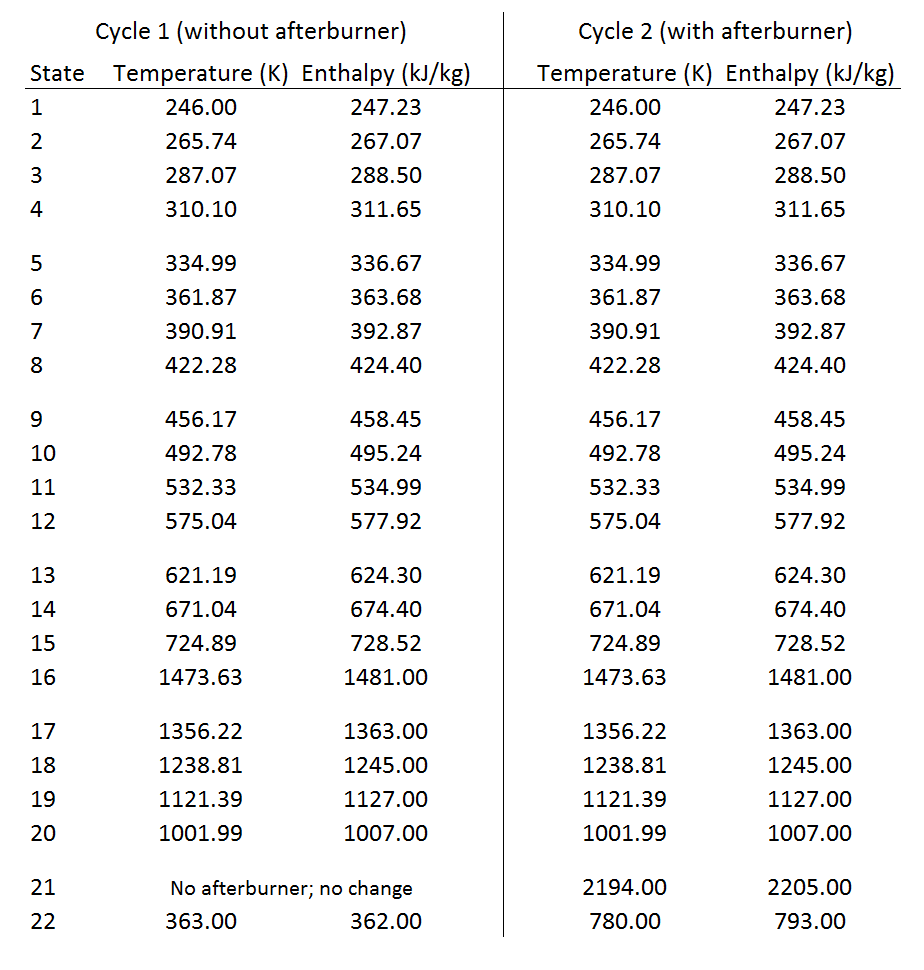
\includegraphics[scale=0.832]{cold_air_data.png}
  \caption{This table lists the temperature (K) and enthalpy $\si{kJ/kg}$ found at every state throughout the cycle for the cold air-standard analysis.}
  \label{fig:cold_air_data}
\end{figure}

\begin{figure}[!hp]
  \centering
  \textbf{Figure 3} State Properties Using Air-standard Analysis\par\medskip
  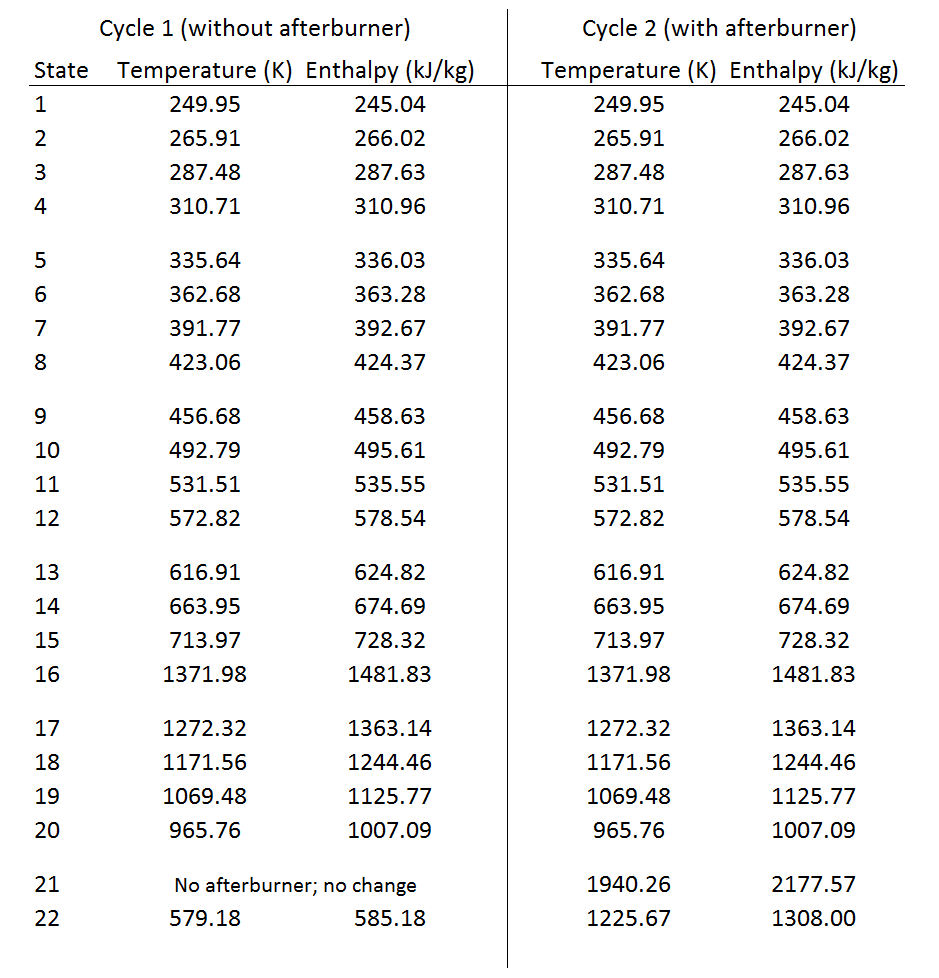
\includegraphics[scale=0.832]{regular_air_data.png}
  \caption{This table lists the temperature (K) and enthalpy $\si{kJ/kg}$ found at every state throughout the cycle for the air-standard analysis.}
  \label{fig:regular_air_data}
\end{figure}

\pagebreak
\subsection*{T-s and P-$\upsilon$ Diagrams}

\begin{figure}[!h]
  \centering
  \textbf{Figure 4} Diagrams for Cold Air-standard Analysis\par\medskip
  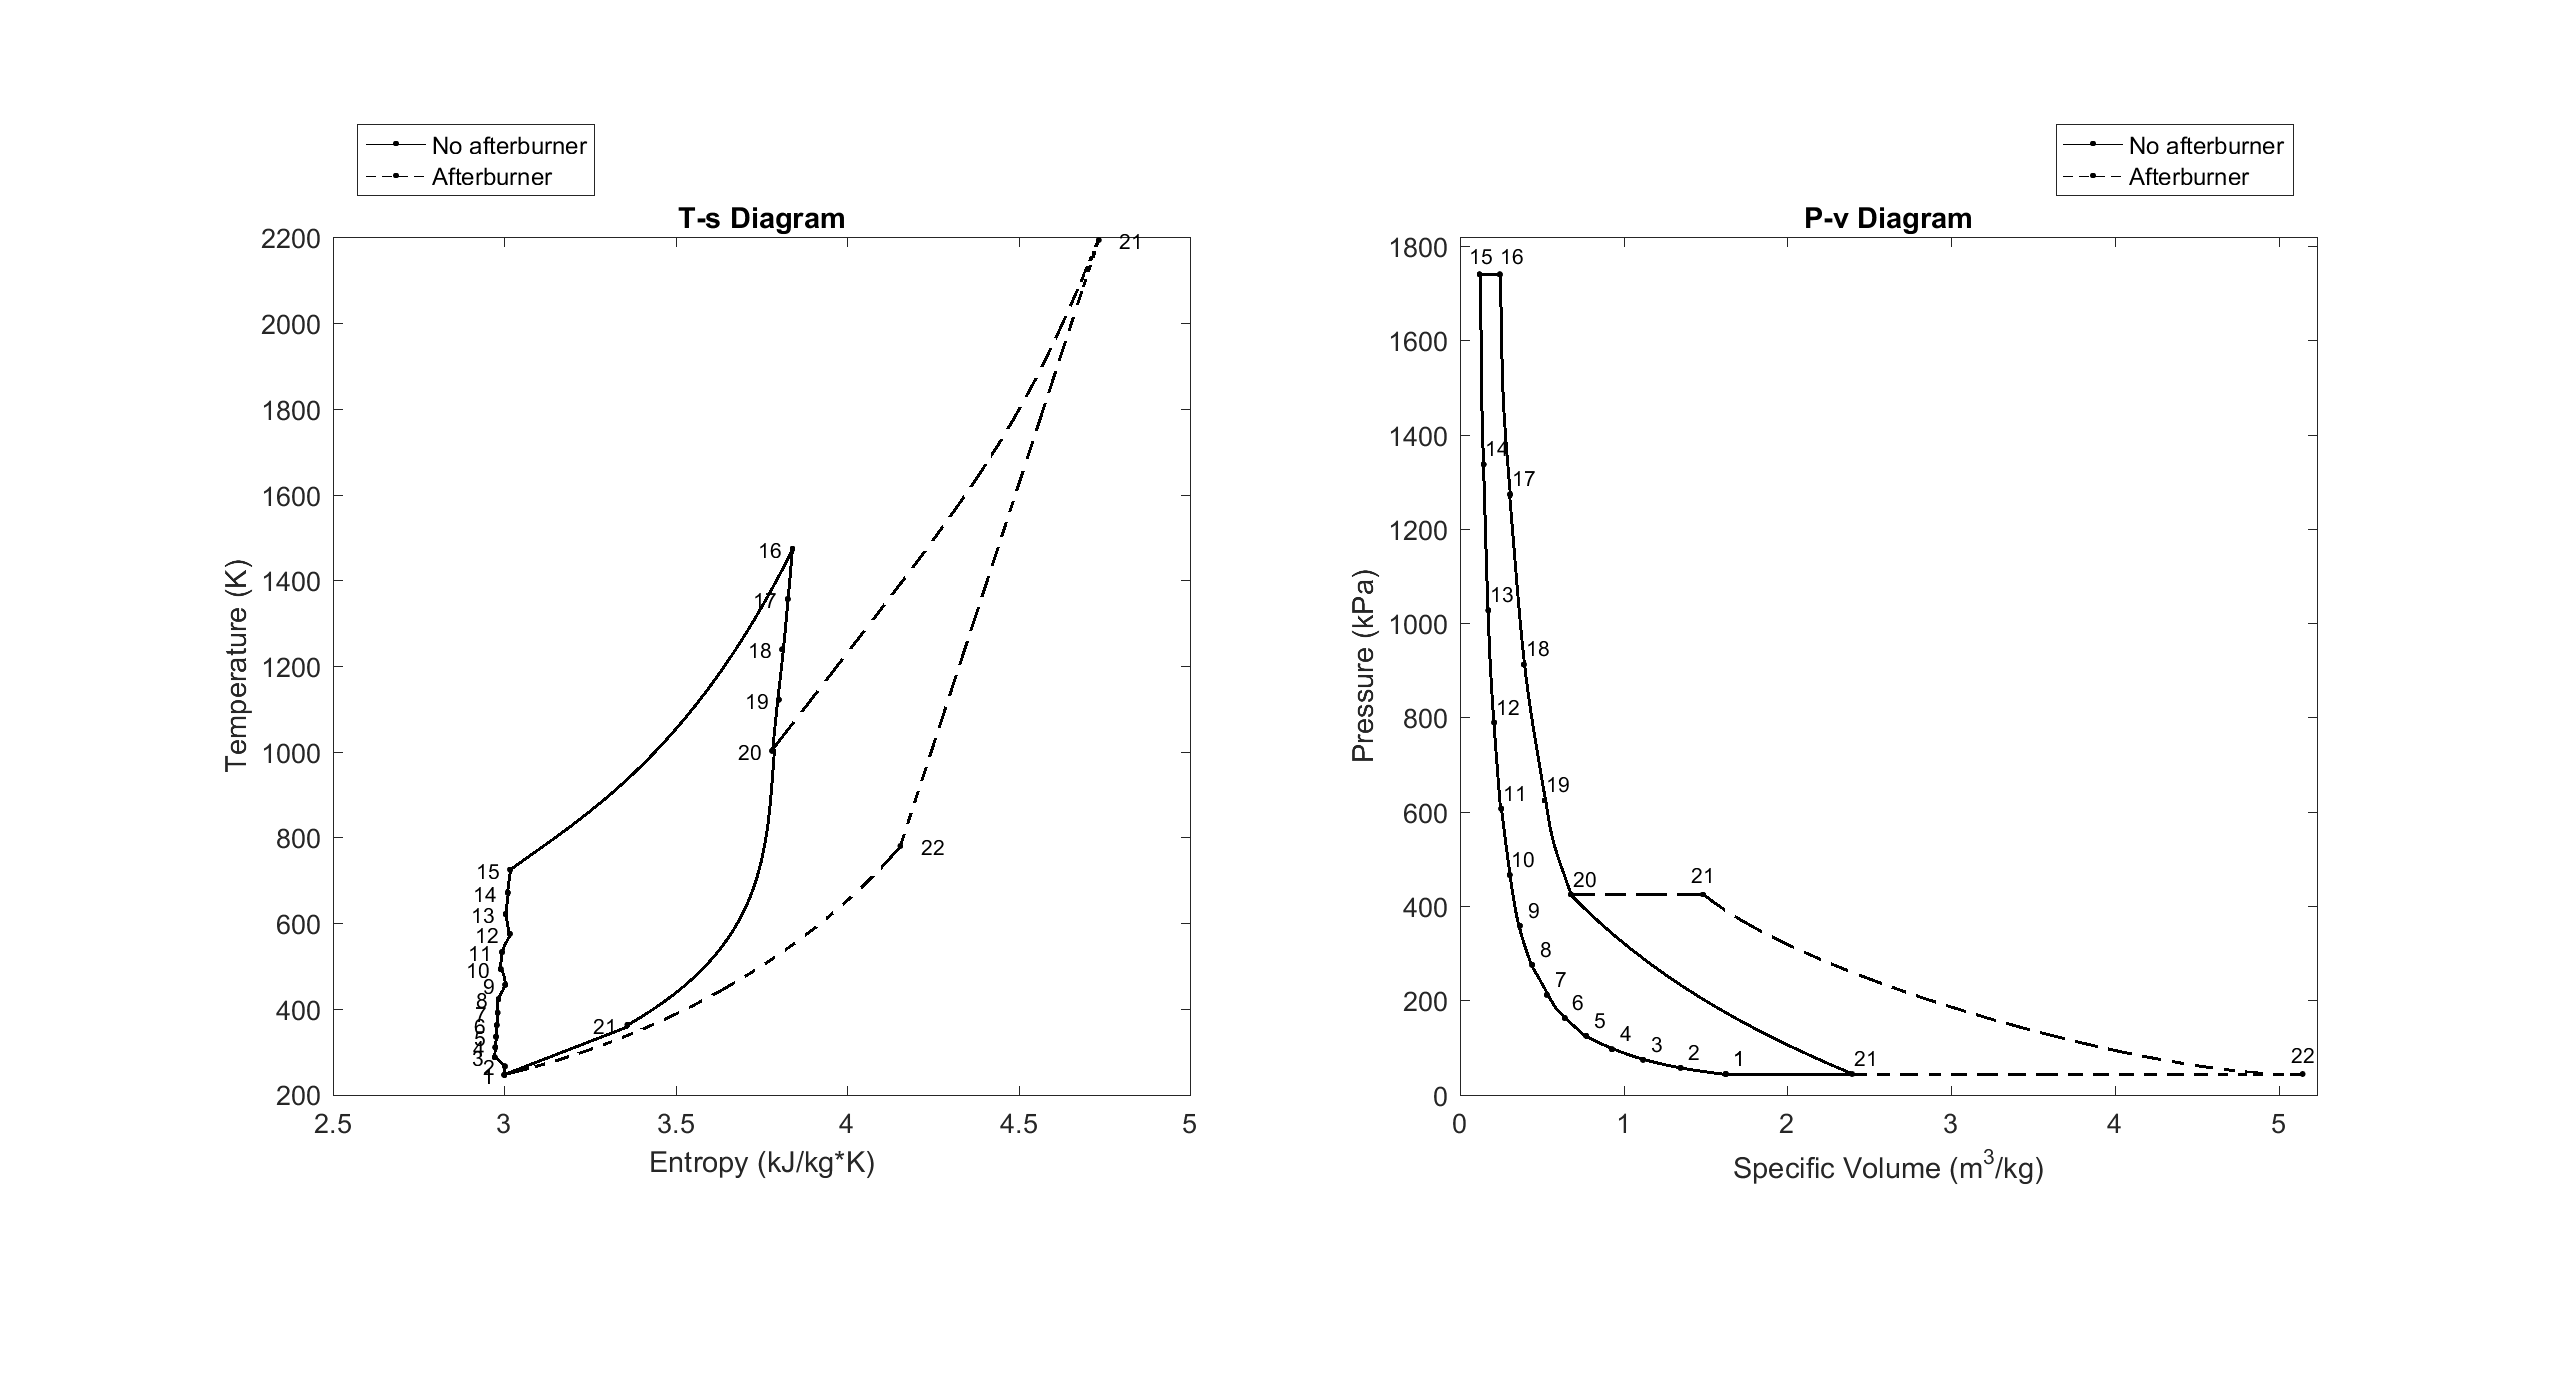
\includegraphics[scale=0.48]{cold_air_diagrams.png}
  \caption{This figure shows both the T-s and P-$\upsilon$ diagrams for the F-100 core using a cold air-standard analysis. For the T-s diagram, the entropy at state 1 was defined to be $-3 \ \si{kJ/kg*K}$ (completely arbitray), and then the temperatures were plotted against the absolute values of all the entropies to produce a graph in the first quadrant.}
  \label{fig:cold_air_diagrams}
\end{figure}

\begin{figure}[!h]
  \centering
  \textbf{Figure 5} Diagrams for Air-standard Analysis\par\medskip
  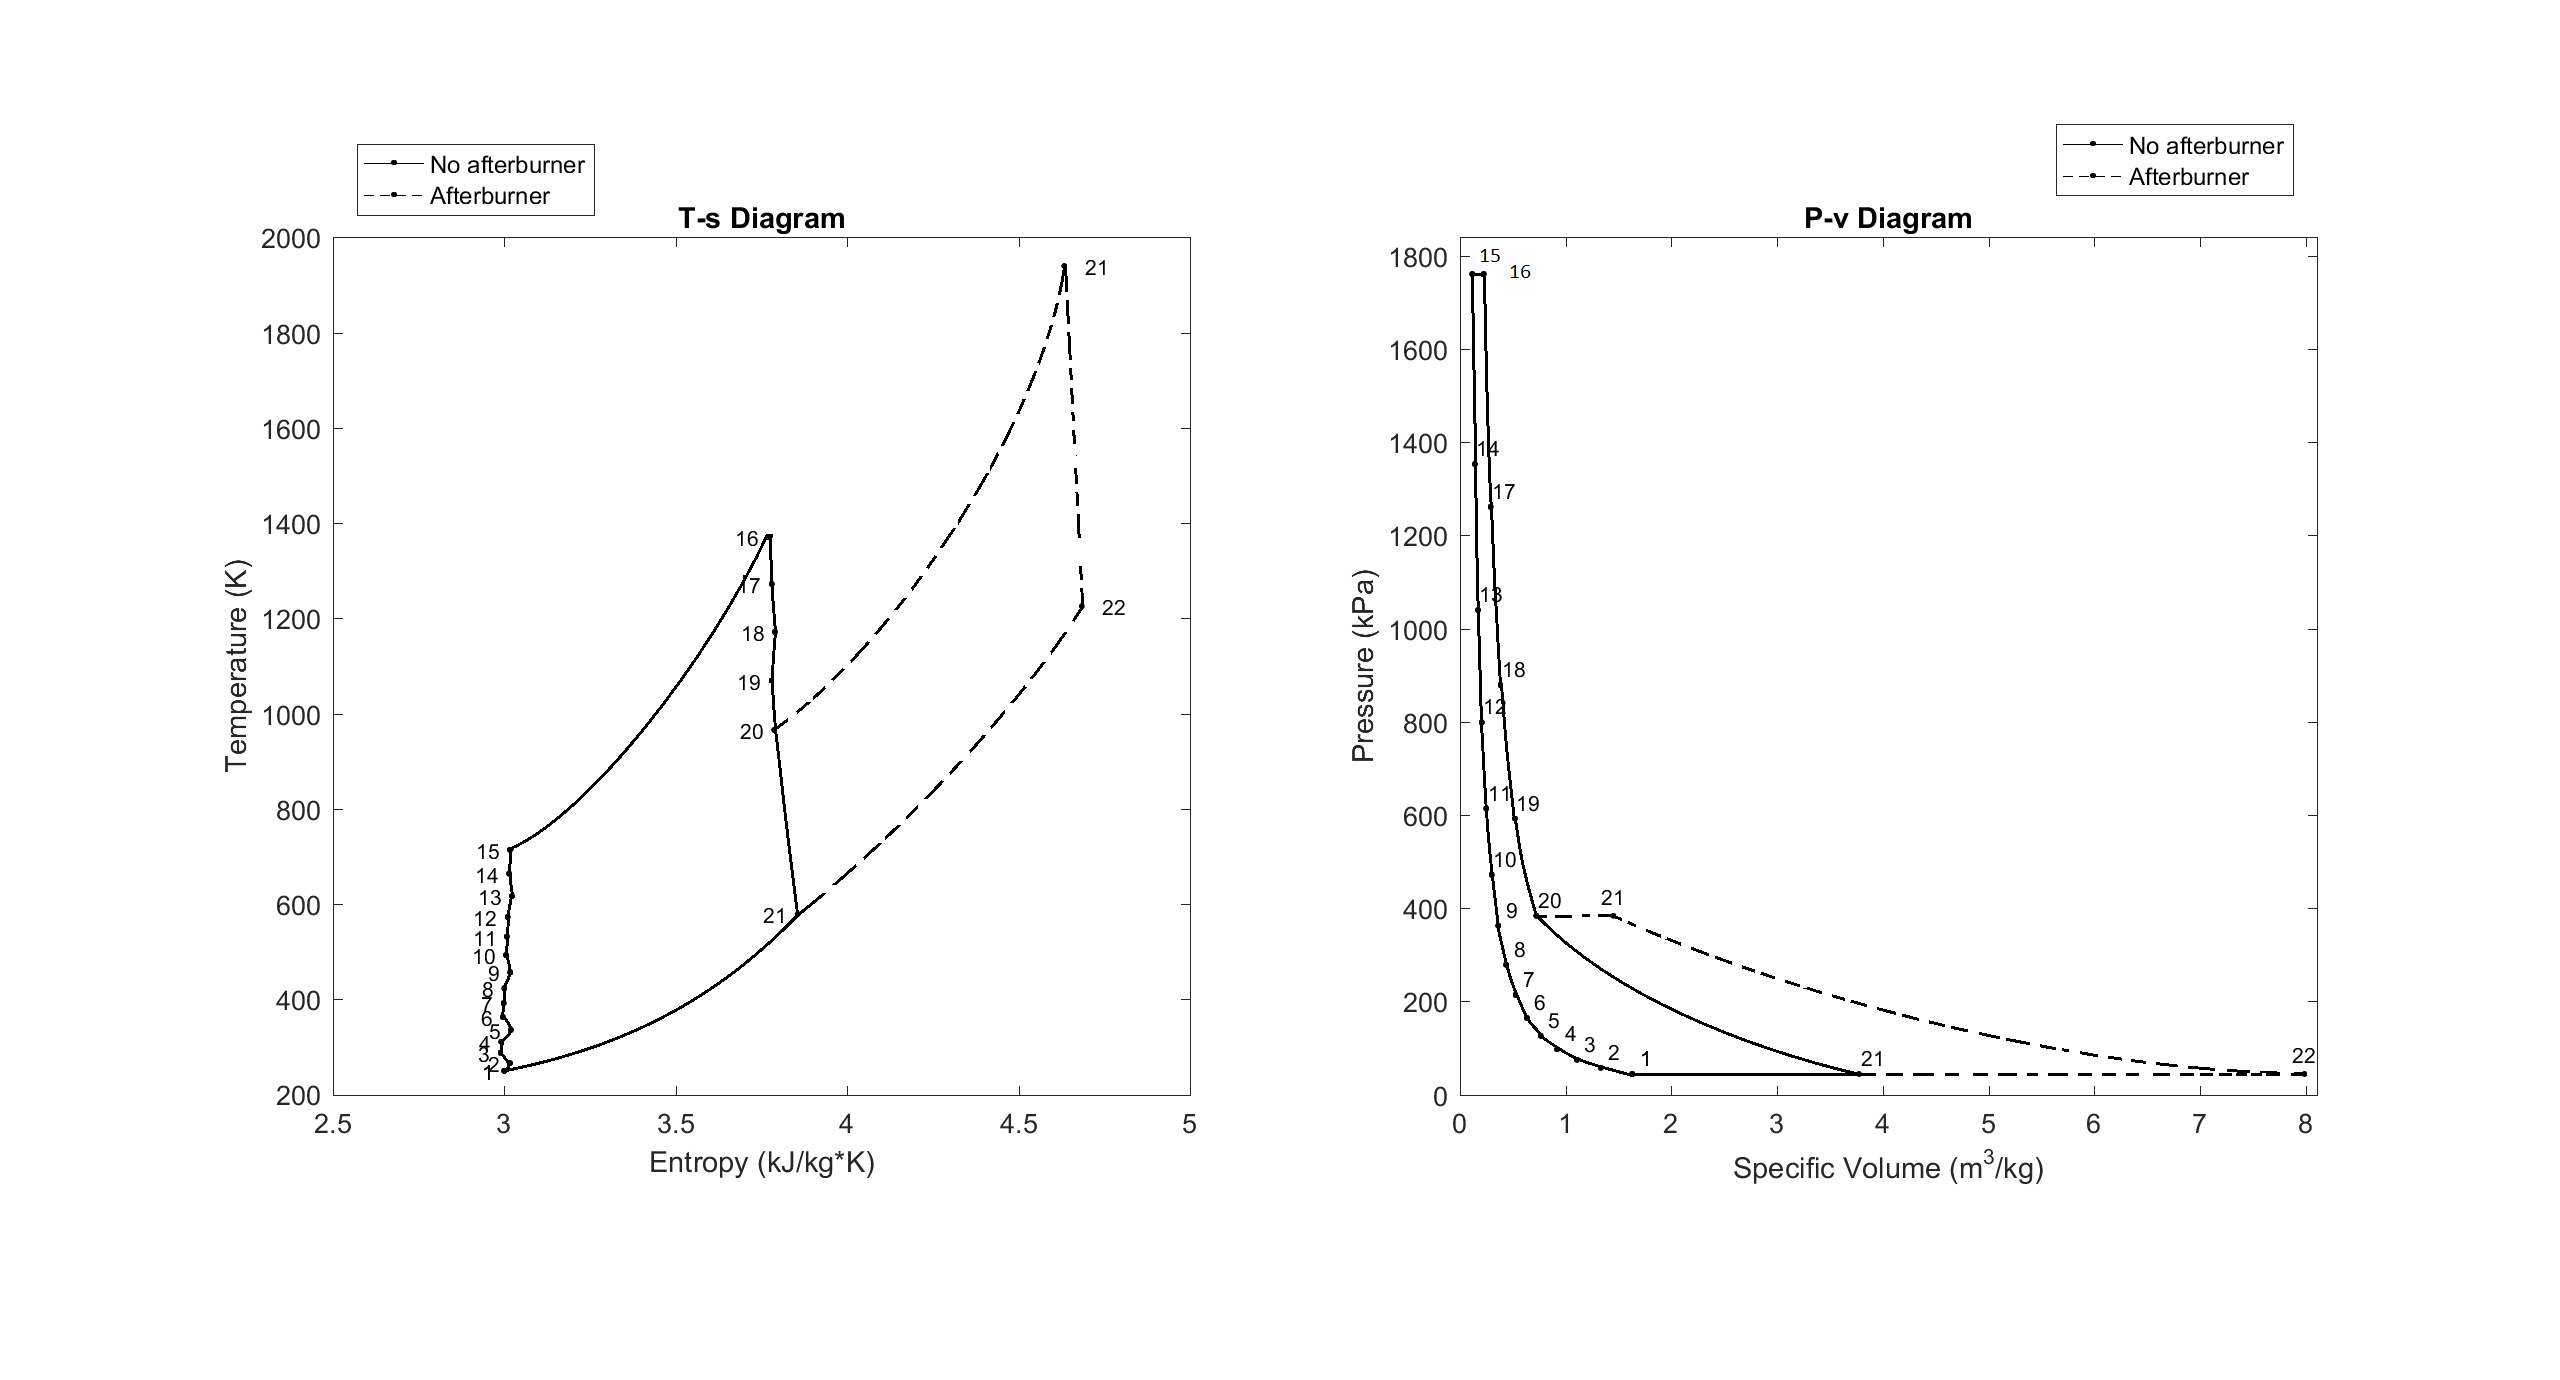
\includegraphics[scale=0.48]{regular_air_diagrams.png}
  \caption{This figure shows both the T-s and P-$\upsilon$ diagrams for the F-100 core using an air-standard analysis. For the T-s diagram, the entropy at state 1 was defined to be $-3 \ \si{kJ/kg*K}$ (completely arbitray), and then the temperatures were plotted against the absolute values of all the entropies to produce a graph in the first quadrant.}
  \label{fig:regular_air_diagrams}
\end{figure}


%----------------------------------------------------------------------------------------
% DISCUSSION
%----------------------------------------------------------------------------------------

\pagebreak
\section{Discussion}
After analyzing both cycles under the cold air-standard and air-standard methods, we found that the air-standard method proved to be more accurate, showing higher values for the temperature at the exit of the nozzle. This is to be expected since the jet engine is operating at an atmospheric temperature outside that of the cold air-standard range. Be that as it may, the T-s and P-$\upsilon$ diagrams in both standards acted as expected, showing the correct rises and falls in the graphs for each piece of the engine, along with increases in entropy and specific volume when the afterburner was used. The only change that could have been made would be to include a diffuser into our analysis process, instead of assuming the ambient air flowed directly into the compressor. Changing this assumption would have made the calculations at the inlet of the compressor more accurate. \\

The use of the afterburner also proved to provide the engine with a higher exit velocity and thus, a larger amount of thrust. However, it would be very unwise for a plane to run both the combustor and afterburner at full throttle, because over two and a half kilograms of fuel would be burned per second. This would result in a very fast depletion of the plane’s fuel.

%----------------------------------------------------------------------------------------
% APPENDICIES
%----------------------------------------------------------------------------------------

\section{Appendicies}

\subsection*{Mass Flow Rate Calculations}
The mass flow rates for the combustor are computed below. Note: The change in cp in the combustor from the mass flow rate of the fuel is negligible due to the fact that there is more air than fuel in the mass flow rate out of the combustor.
\begin{align*}
\dot{m}_{\text{air}} &= \dot{m}_{\text{1}} \\
&= \rho_1 A_{\text{C}} V_{inlet} \\
&= \frac{P_1 (MW)_{air}}{RT_1}A_{\text{C}} V_{inlet} \\
&= \frac{ (43500\ \si{Pa})(28.97\ \si{kg/kmol})}{(8314\ \si{J/kmol\cdot K})(246\ K)}(0.5\ \si{m^2})(166.67\ \si{m/s}) \\
&\approx 50.18\ \si{kg/s} \\\\
\dot{m}_{\text{combustor fuel}} &= 500 + 55\dot{m}_{\text{air}} \\
&= 500 + 55(50.18\ \si{kg/s}) \\
&\approx 3259.9\ \si{kg/hr} \\
&\approx 0.9055\ \si{kg/s} \\\\
\dot{m}_{\text{out combustor}} &= \dot{m}_{\text{combustor fuel}} + \dot{m}_{\text{air}} \\
&= (0.9055\ \si{kg/s}) + (50.18\ \si{kg/s}) \\
&\approx 51.0855\ \si{kg/s} \\\\
\end{align*}

The mass flow rates for the afterburner are computed below. Note: The change in cp in the afterburner from the mass flow rate of the fuel is negligible due to the fact that there is more air than fuel in the mass flow rate out of the afterburner.
\begin{align*}
\dot m_{\text{afterburner fuel}} &= -400 + 110 \dot m_{\text{out combustor}} \\
&= (-400) + (110)(51.0855\ \si{kg/s}) \\
&\approx 5219.504\ \si{kg/hr} \\
&\approx 1.4498\ \si{kg/s}\\\\
\dot m_{\text{afterburner out}} &= \dot m_{\text{afterburner fuel}} + \dot m_{\text{out combustor}} \\
&= (1.4498\ \si{kg/s}) + (51.0855\ \si{kg/s}) \\
&\approx 52.5353\ \si{kg/s}
\end{align*}

\subsection*{Rate of Heat Addition Calculations}
The rates of heat addition for the combustor and afterburner are computed below.
\begin{align*}
\dot{Q}_{\text{in combustor}} &= Q_{in}\dot{m}_{\text{combustor fuel}} \\
&= (43360\ \si{kJ/kg})(0.9055\ \si{kg/s}) \\
&\approx 39262.48\ \si{kJ/s}\\\\
\dot{Q}_{\text{in afterburner}} &= Q_{in}\dot{m}_{\text{afterburner fuel}}\\
&= (43360\ \si{kJ/kg})(1.4498\ \si{kg/s}) \\
&\approx 62863.33\ \si{kJ/s}\\\\
\end{align*}

\end{document}
